% =============================================
% CAPÍTULO 8 - PROTOTIPAGEM DAS TELAS
% =============================================
\chapter{PROTOTIPAGEM DAS TELAS}

Esta seção apresenta as capturas de tela do protótipo funcional da aplicação, desenvolvido com o objetivo de validar os fluxos de interação e a experiência do usuário antes da implementação definitiva. As telas foram elaboradas com foco na usabilidade e na aderência aos requisitos levantados nas etapas anteriores, ilustrando os principais pontos de entrada da plataforma: a tela de boas-vindas e a tela de autenticação. A Figura~\ref{fig:tela_welcome} e a Figura~\ref{fig:tela_authentication} apresentam essas telas respectivamente.

\begin{figure}[H]
    \centering
    \begin{subfigure}[t]{0.45\textwidth}
        \centering
        \caption{Tela de boas-vindas.}
        \label{fig:tela_welcome}
        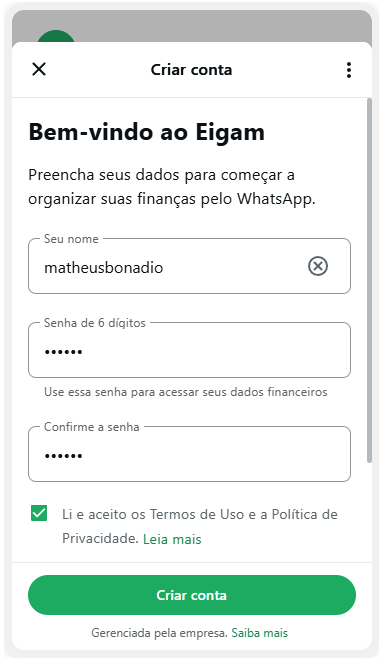
\includegraphics[width=\textwidth]{images/capturas_tela/welcome.png}
    \end{subfigure}
    \hfill
    \begin{subfigure}[t]{0.45\textwidth}
        \centering
        \caption{Tela de autenticação.}
        \label{fig:tela_authentication}
        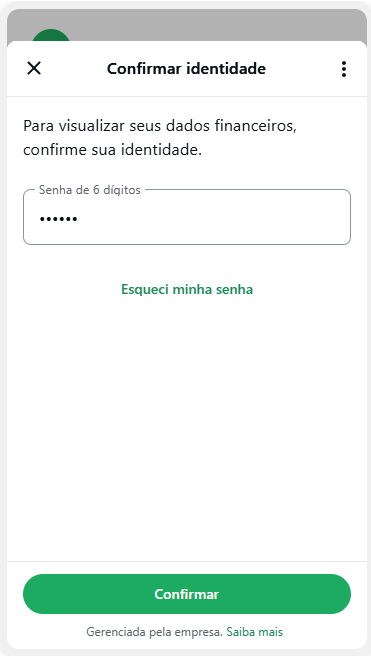
\includegraphics[width=\textwidth]{images/capturas_tela/authentication.png}
    \end{subfigure}
    \fontetabela{\textbf{Fonte:} Elaborado pelos autores (2026).}
\end{figure}
